% =====================================================================
% Agentic AI as a Copilot to Reduce MTTD and MTTR During Incident
% Response: A Systematic Literature Review
% First draft — IEEE journal format (IEEEtran).
% NOTE: for final submission to IEEE Access, swap the class below for the
% official ieeeaccess.cls template (content is compatible).
% Build: pdflatex main && bibtex main && pdflatex main && pdflatex main
% =====================================================================
\documentclass[journal]{IEEEtran}
\usepackage[utf8]{inputenc}
\usepackage[T1]{fontenc}
\usepackage{graphicx}
\usepackage{booktabs}
\usepackage{tikz}
\usetikzlibrary{arrows.meta,positioning,calc}
\usepackage{array}
\usepackage{url}
\usepackage[hidelinks]{hyperref}

\begin{document}

\title{Agentic AI as a Copilot to Reduce MTTD and MTTR During Incident
Response: A Systematic Literature Review}

\author{Valdomiro~de~O.~Souza~Jr.,~\IEEEmembership{Master Degree Student,}
        PPGCA --- Applied Computing Graduate Program, Universidade do Vale
        do Rio dos Sinos (Unisinos), Brazil
% TODO: add advisor as co-author before submission
\thanks{Manuscript drafted October 26, 2026. This work was conducted within
the Applied Computing Graduate Program (PPGCA) at Unisinos, Brazil.}}

\markboth{First draft --- prepared for submission to IEEE Access}%
{Souza Jr.: Agentic AI as a Copilot to Reduce MTTD and MTTR During Incident Response}

\maketitle

\begin{abstract}
Incident response (IR) in modern IT operations is constrained by two
time-based indicators --- Mean Time to Detect (MTTD) and Mean Time to
Recovery (MTTR) --- and by the cognitive load imposed on operations teams
(SRE, NOC, SOC) by alert fatigue and telemetry complexity. Agentic AI
systems, which combine Large Language Models (LLMs) with planning, memory,
tool use, and human supervision, are increasingly proposed as
\emph{copilots} for these teams. This article reports a systematic
literature review (SLR), conducted under the guidelines of Kitchenham et
al.\ and the PRISMA~2020 flow, that consolidates the evidence on Agentic
AI copilots for incident response, with cognitive-load reduction treated
as a complementary outcome. Across two update cycles over a foundational
corpus, 89~candidate studies (2020--2026) were identified and screened,
61 were assessed in full text by \emph{three independent evaluators}
(inter-rater agreement 90.2--91.8\% per pair; Fleiss' $\kappa=0.53$;
53/61 unanimous decisions), and \textbf{53 studies} were included. The
review makes three findings. First, no included study measures MTTD
\emph{and} MTTR nominally against its own baseline in production: the
single study that reports nominal MTTR does so in a proof of concept,
compared against the literature, with results unfavorable to the proposed
agent. Second, the published evidence is dominated by detection proxies
(accuracy, F1, AUC) and qualitative claims, while secondary sources
report dramatic operational gains (e.g., MTTR reduced from 8~hours to 90
minutes) that remain unverified by primary experiments. Third, direct
measurement of operator cognitive load exists in adjacent domains
(neuroergonomics, control rooms, maritime operations) but has never been
combined with an agentic copilot in IT incident response. These gaps
jointly define a concrete research agenda: field evaluations of agentic
copilots instrumented for nominal MTTD/MTTR with their own baselines and
validated cognitive-load instruments.
\end{abstract}

\begin{IEEEkeywords}
Agentic AI, AIOps, incident response, LLM agents, MTTD, MTTR, cognitive
load, multi-agent systems, systematic literature review, SOC.
\end{IEEEkeywords}

\IEEEpeerreviewmaketitle

% =====================================================================
\section{Introduction}
\label{sec:intro}

\IEEEPARstart{M}{odern} IT operations teams face a structural asymmetry:
distributed, cloud-native systems generate telemetry at machine speed,
while detection, diagnosis, and remediation remain bounded by human
cognition. The operational cost of this asymmetry is captured by two
indicators --- \emph{Mean Time to Detect} (MTTD) and \emph{Mean Time to
Recovery} (MTTR) --- and by a human cost that is harder to see on
dashboards: alert fatigue and sustained cognitive load on SRE, NOC, and
SOC personnel. Industry reports cited in the corpus place average breach
identification and containment at 277~days (204 to detect, 73 to
contain)~\cite{P79}, while SOC analysts discard the majority of alerts as
false positives.

\emph{Agentic AI} --- AI systems that pursue goals with some degree of
autonomy by combining LLM-based reasoning with planning, memory, tool
use, and human oversight~\cite{P09,P10} --- has been proposed as a new
operating model for incident response: not full automation, but a
\emph{copilot} that perceives, reasons, acts, and learns alongside the
human operator. The promise is threefold: earlier detection (MTTD),
faster remediation (MTTR), and a lighter day-to-day workload for
operations teams.

This article asks whether the published evidence supports that promise.
It reports a systematic literature review (SLR) conducted under the
guidelines of Kitchenham et al.~\cite{kitchenham2009}, with study
selection reported in the PRISMA~2020 format~\cite{page2021prisma}, scope
delimited with the PICOC framework~\cite{petticrew2006}, and quality
assessment mirroring the DARE criteria~\cite{dare}. The review was
executed as an \emph{update review} in two cycles over a foundational
corpus of 19 studies, processing 89 candidate studies in total, and ---
unusually for SLRs in this area --- every full-text assessment was
performed independently by \emph{three evaluators}, with inter-rater
reliability quantified by Cohen's~\cite{cohen1960} and
Fleiss'~\cite{fleiss1971} kappa.

The contributions are:
\begin{enumerate}
  \item a consolidated corpus of 53 studies (2020--2026) on Agentic AI
        for incident response and adjacent IT operations, organized in a
        taxonomy of agentic paradigms (Section~\ref{sec:results});
  \item triple-verified bibliometrics (OpenAlex, Crossref, Scopus) and an
        internal cross-citation map of the corpus (52 citing edges)
        identifying its conceptual hubs;
  \item evidence synthesis showing that \textbf{no study measures MTTD
        and MTTR nominally with its own baseline in production}
        (Section~\ref{sec:mttr}), and a catalogue of the proxies actually
        used;
  \item a bridge to the human-factors literature: a cluster of studies
        that measure operator cognitive load directly --- yet never in
        combination with an agentic copilot in IT incident response
        (Section~\ref{sec:cogload});
  \item a methodological contribution: a fully reproducible three-rater
        protocol whose residual disagreements (8 of 61 decisions) are all
        traceable to three explicit protocol rules rather than to content
        interpretation (Section~\ref{sec:reliability}).
\end{enumerate}

% =====================================================================
\section{Background and Related Work}
\label{sec:background}

\subsection{From AIOps to Agentic AI}
AIOps applies machine learning to IT operations data --- logs, metrics,
traces --- for anomaly detection, root cause analysis (RCA), and
remediation. Surveys in the corpus trace its evolution from
knowledge-based automation to ML pipelines~\cite{P16} and, after 2023,
to LLM-centered architectures~\cite{P05}. The agentic turn adds goal
pursuit under governance: taxonomies distinguish \emph{AI agents}
(tool-using, single-task) from \emph{Agentic AI} (multi-step autonomy
with planning and memory)~\cite{P09}, and reference surveys map its
technologies, applications, and societal implications~\cite{P10,P15,P54}.

\subsection{Incident response and its metrics}
Incident response spans detection, triage, diagnosis (RCA), remediation,
and post-incident learning. MTTD and MTTR are its canonical outcome
metrics; alert fatigue and operator cognitive load are its canonical
human costs. In security operations, the same cycle appears as SOC
triage and SOAR playbooks~\cite{P28,P79}. A persistent finding of this
review --- anticipated here --- is that primary studies rarely
instrument these nominal metrics, reporting detection-quality proxies
instead.

\subsection{The foundational corpus and its hubs}
The present review updates a foundational SLR (19 studies, P01--P19).
Cross-citation analysis over the full corpus (Section~\ref{sec:cross})
shows that three foundational surveys act as conceptual hubs ---
\cite{P10} (7 internal citations), \cite{P09} (6), and \cite{P14} (5) ---
confirming their role as the definitional substrate on which the
empirical studies build.

% =====================================================================
\section{Review Method}
\label{sec:method}

The protocol follows Kitchenham et al.~\cite{kitchenham2009}: planning
(PICOC, research questions, search string), conducting (search,
screening, quality assessment, extraction), and reporting (this
article). All protocol artifacts --- prompts, extraction sheets,
per-study assessments, and machine-readable result tables --- are
version-controlled in the research repository.

\subsection{PICOC}
\label{sec:picoc}

Table~\ref{tab:picoc} shows the PICOC delimitation~\cite{petticrew2006}.
A protocol rule (v1.1.0), introduced after a three-rater calibration of
the PICOC extraction itself, requires that \emph{Comparison} be recorded
as declared \textbf{only when the study executes an empirical comparison
against a concrete baseline}; purely conceptual contrasts (e.g.,
``Agentic AI vs.\ traditional AI'' in prose) are recorded as not
applicable. This rule removed 100\% of the inter-rater divergences
observed in the Comparison field.

\begin{table}[!t]
\caption{PICOC delimitation of the review.}
\label{tab:picoc}
\centering
\begin{tabular}{@{}p{0.22\columnwidth}p{0.68\columnwidth}@{}}
\toprule
\textbf{Element} & \textbf{Definition} \\
\midrule
Population & Complex software systems and the teams operating them
(SRE, NOC, SOC); microservices; IT operations pipelines. \\
Intervention & Agentic AI as copilot or autonomous agent:
LLM-based agents, multi-agent systems, LLM4AIOps, the
perceive--reason--act--learn loop. \\
Comparison & Traditional automation, non-agentic AIOps, or human
baselines --- \emph{declared only with an executed empirical baseline}
(rule v1.1.0). \\
Outcomes & MTTD, MTTR, observability, detection accuracy,
alert fatigue, and operator cognitive load (complementary outcome). \\
Context & The incident-response life cycle in IT operations and
cybersecurity; HITL/HOTL supervision; production vs.\ simulation. \\
\bottomrule
\end{tabular}
\end{table}

\subsection{Research questions}
\label{sec:rqs}

\begin{itemize}
  \item \textbf{RQ1 (Context/Definitions).} Which capabilities and
        autonomy levels (planning, memory, tool use, human supervision)
        characterize Agentic AI, and how do they affect decision-making
        in complex environments?
  \item \textbf{RQ2 (Engineering/Architecture).} Which architectures and
        mechanisms (orchestration, memory, tools, guardrails,
        observability) sustain Agentic AI in production?
  \item \textbf{RQ3 (Evidence/Benefits).} Which quantitative and
        qualitative evidence reports benefits, and which metrics are
        used (response time, decision quality, operational load),
        especially in incident response?
  \item \textbf{RQ4 (Challenges/Ethics).} Which risks and challenges
        (security, robustness, governance, accountability) limit
        responsible use in critical systems?
  \item \textbf{RQ5 (Gaps).} Which gaps and future directions
        (evaluation/benchmarking, threat models, governance,
        observability, alignment) are identified?
\end{itemize}

\subsection{Search and identification}
The search string was derived from the cross-study PICOC synthesis as
two mandatory blocks --- \emph{Intervention} (agentic AI, LLM agents,
multi-agent systems, AIOps copilots) AND \emph{Context/Population}
(incident response, IT operations, SRE/NOC/SOC, observability) ---
with \emph{Outcomes} deliberately optional, since only 1 of 38 calibration
studies named MTTD/MTTR in its metadata. The string was calibrated
against the known corpus and validated by real execution on OpenAlex
($\approx$49{,}700 records) and on the Scopus Search API (12{,}783
records, 2020+, English), achieving 13/14 recall of the included
calibration set in both engines with the same single miss. Candidate
identification combined assisted search (cycle~1: three independent LLM
assistants, $\approx$51 raw records) and author-driven discovery
(cycle~2: 49 candidates). Backward/forward snowballing is mandatory in
the protocol because one included study is not indexed by Scopus and one
is not retrieved by the main query.

\subsection{Selection criteria}
Inclusion required: publication year $\geq$2020 (I1); an identifiable
peer-reviewed venue (I2); venue quality thresholds (I3--I4, national
Qualis A1--A2 and SJR Q1--Q2); at least one citation in any of three
indexers, with a recency exception for papers younger than 12~months
(I5); and thematic adherence --- an \emph{agentic} approach in the
\emph{IR/AIOps/SOC} domain (I6). Exclusion criteria: sub-threshold venue
strata (E1), non-agentic approaches (E2), out-of-domain studies (E3),
duplicates (E4), and non-peer-reviewed material (E5). A dated protocol
amendment in cycle~2 allowed four candidates outside the I3/I4 strata to
proceed to full-text assessment \emph{with a mandatory stratum caveat};
the amendment is itself part of the audit trail and, notably, is the
root cause of three of the eight residual inter-rater divergences
(Section~\ref{sec:reliability}).

\subsection{Selection flow (PRISMA)}
\label{sec:prisma}

Fig.~\ref{fig:prisma} shows the PRISMA~2020 flow of both update cycles
over the foundational corpus, and Table~\ref{tab:prisma} summarizes the
stage counts side by side. In cycle~2,
thematic exclusion (E2/E3) was applied already at screening, because a
full-text PICOC extraction of all 49 candidates (one reading agent per
PDF, consolidated and audited) provided per-study evidence before
assessment --- each screening exclusion cites that evidence and a
cycle-1 precedent.

\begin{figure*}[!t]
\centering
\resizebox{\textwidth}{!}{%
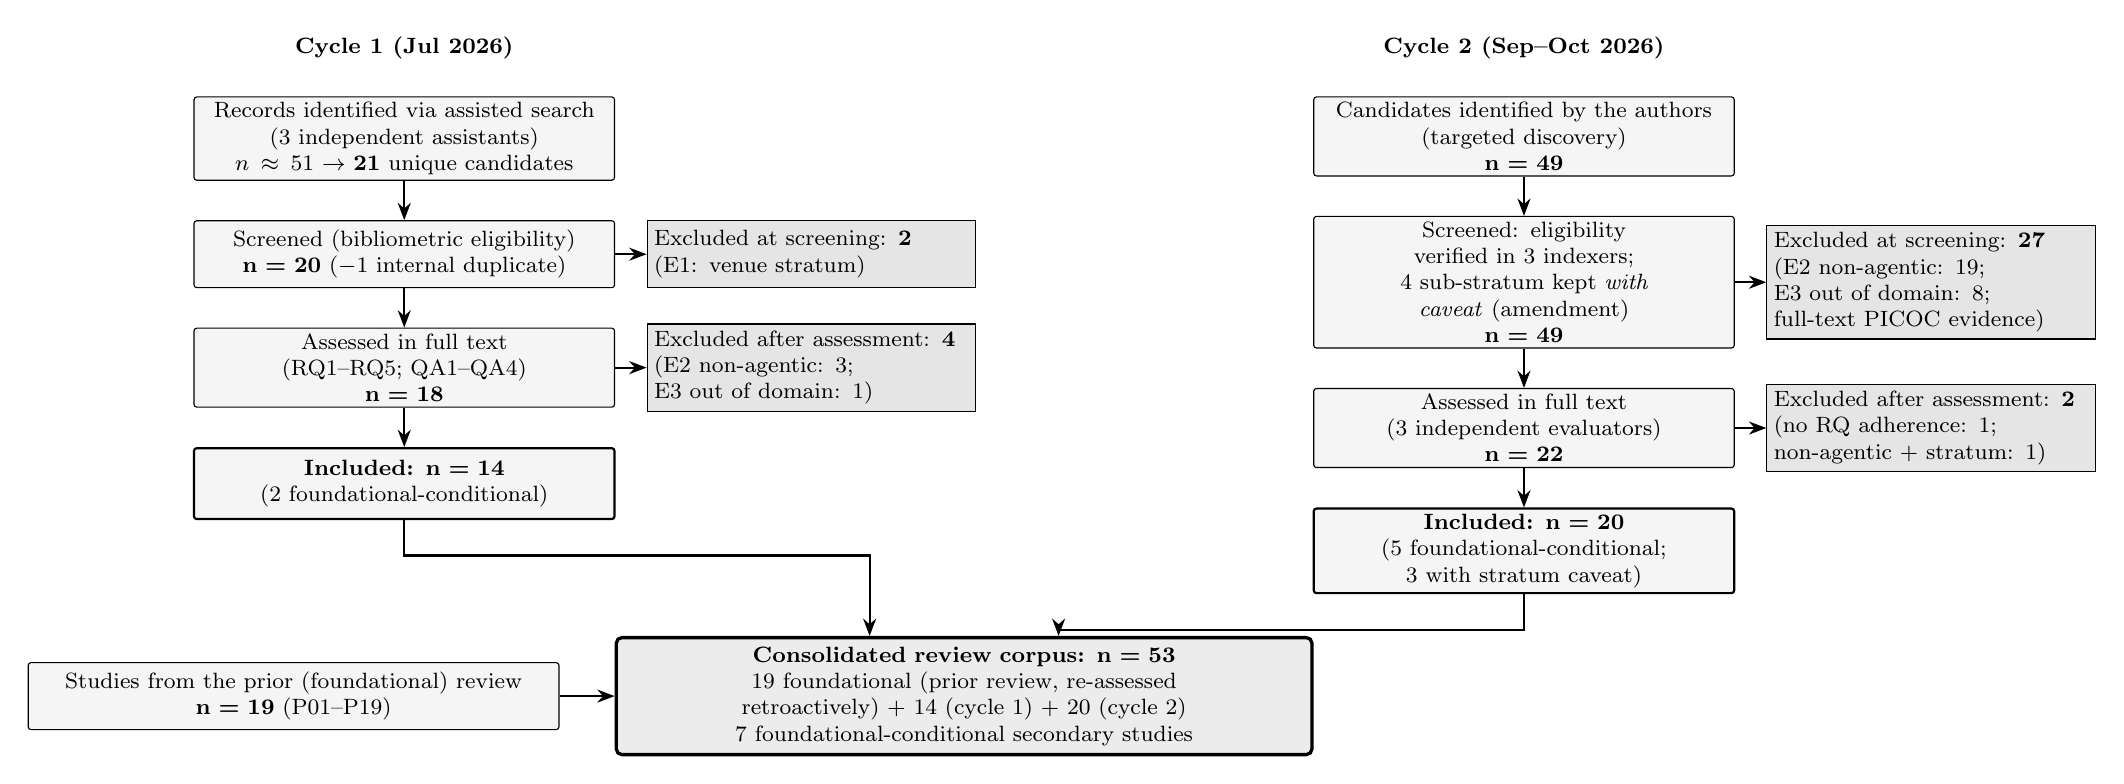
\begin{tikzpicture}[
  font=\footnotesize,
  box/.style={draw, rounded corners=1pt, align=center, fill=gray!8,
              minimum height=8.5mm, text width=52mm, inner sep=2pt},
  excl/.style={draw, align=left, fill=gray!20, minimum height=8.5mm,
               text width=40mm, inner sep=2.5pt},
  incl/.style={draw, thick, rounded corners=1pt, align=center, fill=gray!8,
               minimum height=9mm, text width=52mm, inner sep=2pt},
  final/.style={draw, very thick, rounded corners=2pt, align=center,
                fill=gray!15, minimum height=11mm, text width=86mm},
  lbl/.style={font=\footnotesize\bfseries\scshape},
  arr/.style={-{Stealth[length=2.2mm]}, thick}
]
% ---------------- Cycle 1 column ----------------
\node[lbl] (c1t) {Cycle 1 (Jul 2026)};
\node[box, below=3.5mm of c1t] (c1a)
  {Records identified via assisted search\\(3 independent assistants)\\
   $n\approx51$ $\rightarrow$ \textbf{21} unique candidates};
\node[box, below=5mm of c1a] (c1b)
  {Screened (bibliometric eligibility)\\\textbf{n = 20} ($-1$ internal duplicate)};
\node[excl, right=4mm of c1b.east, anchor=west] (c1bx)
  {Excluded at screening: \textbf{2}\\(E1: venue stratum)};
\node[box, below=5mm of c1b] (c1c)
  {Assessed in full text\\(RQ1--RQ5; QA1--QA4)\\\textbf{n = 18}};
\node[excl, right=4mm of c1c.east, anchor=west] (c1cx)
  {Excluded after assessment: \textbf{4}\\(E2 non-agentic: 3;\\E3 out of domain: 1)};
\node[incl, below=5mm of c1c] (c1d)
  {\textbf{Included: n = 14}\\(2 foundational-conditional)};
\draw[arr] (c1a) -- (c1b);
\draw[arr] (c1b) -- (c1c);
\draw[arr] (c1c) -- (c1d);
\draw[arr] (c1b.east) -- (c1bx.west);
\draw[arr] (c1c.east) -- (c1cx.west);
% ---------------- Cycle 2 column ----------------
\node[lbl, right=108mm of c1t] (c2t) {Cycle 2 (Sep--Oct 2026)};
\node[box, below=3.5mm of c2t] (c2a)
  {Candidates identified by the authors\\(targeted discovery)\\\textbf{n = 49}};
\node[box, below=5mm of c2a] (c2b)
  {Screened: eligibility verified in 3 indexers;\\
   4 sub-stratum kept \emph{with caveat} (amendment)\\\textbf{n = 49}};
\node[excl, right=4mm of c2b.east, anchor=west] (c2bx)
  {Excluded at screening: \textbf{27}\\(E2 non-agentic: 19;\\E3 out of domain: 8;\\
   full-text PICOC evidence)};
\node[box, below=5mm of c2b] (c2c)
  {Assessed in full text\\(3 independent evaluators)\\\textbf{n = 22}};
\node[excl, right=4mm of c2c.east, anchor=west] (c2cx)
  {Excluded after assessment: \textbf{2}\\(no RQ adherence: 1;\\non-agentic + stratum: 1)};
\node[incl, below=5mm of c2c] (c2d)
  {\textbf{Included: n = 20}\\(5 foundational-conditional;\\3 with stratum caveat)};
\draw[arr] (c2a) -- (c2b);
\draw[arr] (c2b) -- (c2c);
\draw[arr] (c2c) -- (c2d);
\draw[arr] (c2b.east) -- (c2bx.west);
\draw[arr] (c2c.east) -- (c2cx.west);
% ---------------- Foundational + final corpus ----------------
\node[final, below=10mm of $(c1d.south)!0.5!(c2d.south)$] (corpus)
  {\textbf{Consolidated review corpus: n = 53}\\
   19 foundational (prior review, re-assessed retroactively)
   $+$ 14 (cycle 1) $+$ 20 (cycle 2)\\
   7 foundational-conditional secondary studies};
\node[box, text width=66mm, left=7mm of corpus.west, anchor=east, yshift=0mm] (found)
  {Studies from the prior (foundational) review\\\textbf{n = 19} (P01--P19)};
\draw[arr] (c1d.south) -- ++(0,-4.5mm) -| ([xshift=-12mm]corpus.north);
\draw[arr] (c2d.south) -- ++(0,-4.5mm) -| ([xshift=12mm]corpus.north);
\draw[arr] (found.east) -- (corpus.west);
\end{tikzpicture}%
}
\caption{PRISMA~2020 flow of the two update cycles over the foundational
corpus (adapted for a review update). Cycle-2 screening exclusions are
anchored in a full-text PICOC extraction of all 49 candidates; the
stratum amendment is dated and auditable in the protocol.}
\label{fig:prisma}
\end{figure*}

\begin{table}[!t]
\caption{Selection flow across the two update cycles.}
\label{tab:prisma}
\centering
\begin{tabular}{@{}lcc@{}}
\toprule
\textbf{Stage} & \textbf{Cycle 1} & \textbf{Cycle 2} \\
\midrule
Identified                 & $\approx$51 $\rightarrow$ 21 unique & 49 \\
Screened                   & 20 (--1 duplicate)      & 49 \\
Excluded at screening      & 2 (E1)                  & 27 (E2=19, E3=8) \\
Assessed in full text      & 18                      & 22 \\
Excluded after assessment  & 4                       & 2 \\
\textbf{Included}          & \textbf{14}             & \textbf{20} \\
Corpus (cumulative)        & 33 (19+14)              & \textbf{53} (33+20) \\
\bottomrule
\end{tabular}
\end{table}

The 53-study corpus comprises the 19 foundational studies, 14 cycle-1
inclusions, and 20 cycle-2 inclusions; seven of these are secondary
``foundational-conditional'' studies
\cite{P24,P33,P52,P54,P72,P77,P79} that migrate to background material
if the protocol is restricted to primary studies (primary corpus: 46).

\subsection{Quality assessment and extraction}
Each assessed study received: (i)~a verified bibliometric record
(DOI, venue, year, and citation counts kept \emph{per source} ---
OpenAlex, Crossref, Scopus --- never summed, with ``not indexed''
distinguished from zero); (ii)~an RQ-coverage score (RQ1--RQ5, each
rated fully/partially/not answered = 1.0/0.5/0.0, max 5.0); (iii)~a
DARE-style quality score (QA1 clear objectives, QA2 replicable
methodology, QA3 solid evidence base, QA4 coherent conclusions; max
4.0; bands High $\geq$3.0, Medium 1.5--2.5, Low $<$1.5); and (iv)~an
11-field structured extraction sheet with per-claim evidence anchors
(section/page). The 19 foundational studies were re-assessed
retroactively under the same rubric --- without re-opening their
inherited inclusion --- so that all 61 assessments are directly
comparable.

\subsection{Three-evaluator protocol}
Every full-text assessment was executed independently by three LLM-based
evaluators (Claude, ChatGPT, Gemini) from the same written prompt and
PDF. Agreement was computed on collapsed include/exclude decisions with
Cohen's $\kappa$ per pair~\cite{cohen1960} and Fleiss' $\kappa$ overall
\cite{fleiss1971}. Results are reported in
Section~\ref{sec:reliability}.

% =====================================================================
\section{Results}
\label{sec:results}

\subsection{Corpus overview and taxonomy}
\label{sec:taxonomy}

Table~\ref{tab:taxonomy} organizes the 53 included studies by agentic
paradigm. Three observations structure the corpus. First, the
\emph{foundational layer} is dominated by definitional surveys
\cite{P09,P10,P15,P54} and governance/trust reviews \cite{P01,P17};
these answer RQ1/RQ4/RQ5 strongly but contribute no empirical benefit
evidence. Second, the \emph{empirical core} is concentrated in cycle~1:
multi-agent LLM systems for RCA and SOC \cite{P27,P28,P31,P35},
closed-loop remediation \cite{P22}, and a small-language-model agent for
ICT operations \cite{P21} --- the methodological high-water marks of the
corpus (QA $4.0/4.0$). Third, cycle~2 adds the copilot pattern proper
--- RAG-based security copilots \cite{P78,P83,P87} and SOC
hyper-automation \cite{P76} --- plus a \emph{human-factors cluster}
absent from earlier cycles \cite{P62,P63,P69,P81}.

\begin{table}[!t]
\caption{Taxonomy of the included corpus (n=53; representative studies).}
\label{tab:taxonomy}
\centering
\begin{tabular}{@{}p{0.44\columnwidth}p{0.44\columnwidth}@{}}
\toprule
\textbf{Paradigm} & \textbf{Studies} \\
\midrule
LLM multi-agent (RCA/SOC) & \cite{P27,P28,P31,P35,P76} \\
Single-agent LLM copilot (+RAG) & \cite{P34,P78,P83,P87} \\
Closed-loop remediation agents & \cite{P20,P22,P32} \\
SLM/compact-model agents & \cite{P21} \\
MAS/RL and self-organization (non-LLM) & \cite{P25,P88} \\
Conceptual agentic frameworks (AIOps/PdM) & \cite{P43,P82} \\
AI-assisted SIEM / alert triage & \cite{P73} \\
Foundational surveys (agents, LLM-sec, AIOps) &
\cite{P05,P09,P10,P14,P15,P16,P24,P33,P52,P54,P72,P77,P79} \\
Human factors \& instruments & \cite{P37,P62,P63,P69,P81} \\
\bottomrule
\end{tabular}
\end{table}

\subsection{RQ coverage and quality}
RQ coverage shifted between cycles in a telling way. In cycle~1
(18 assessed; mean RQ score 3.83, mean QA 3.50) the systematic gap was
\textbf{RQ4} (ethics and governance: only 4/18 fully answered). In
cycle~2 (22 assessed; mean RQ 3.16, mean QA 2.75; zero unconditional
inclusions) the gap moved to \textbf{RQ3/QA3}: abundant conceptual
contribution with scarce empirical benefit evidence. The retroactive
assessment of the foundational studies (mean RQ 3.66, mean QA 2.53)
shows the same profile --- high RQ coverage by surveys, low QA for lack
of their own validation. Across all 61 assessments the pattern is
stable: \emph{the literature is conceptually rich and empirically thin
precisely on the benefit claims that motivate it}.

\subsection{Evidence on MTTD and MTTR}
\label{sec:mttr}

This is the review's central result. After screening 89 candidates and
assessing 61 in full text across two cycles:

\begin{itemize}
  \item \textbf{No study measures MTTD and MTTR nominally against its
        own baseline in production.}
  \item \textbf{One study reports nominal MTTR.} The SOC
        hyper-automation agent of~\cite{P76} reports per-phase
        remediation times of $\approx$1--1.5~min in a proof of concept
        (one use case, SSH brute force), compared against
        \emph{literature values} for a commercial security copilot
        ($\approx$30--45~s) --- i.e., no own baseline, and a result
        \emph{unfavorable} to the proposed agent. The authors' candor is
        valuable; the evidence level is PoC.
  \item \textbf{Secondary evidence reports dramatic gains.} The SOC
        survey~\cite{P79} relays primary reports of MTTR reduced from
        8~hours to 90~minutes, 98\% of alerts auto-triaged with
        containment under 5~minutes, and a 277-day industry
        detect-and-contain baseline. None of these numbers is reproduced
        by a primary study in the corpus.
  \item \textbf{Proxies dominate.} The strongest quantified operational
        outcomes are proxies: a 74--84\% global alert-volume reduction in
        a national SOC~\cite{P73}; operator reaction time falling from
        $\approx$276~s to $\approx$107~s with decision support in a
        control-room experiment (Wilcoxon $p<0.01$)~\cite{P81};
        end-to-end incident-report latency of 2.9--11.6~s with 0.3~s
        pre-detection~\cite{P87}; and copilot answer quality
        (BERTScore $\approx$85--87\%) without timing~\cite{P83}.
        Detection studies report accuracy/F1/AUC only.
\end{itemize}

The gap is therefore not merely ``few studies'': it is a structural
mismatch between the motivating claim of the field (time-metric
reduction) and its measurement practice (detection proxies and
qualitative assertions). The claim that agentic copilots reduce MTTD and
MTTR is, as of 2026, \emph{plausible but unverified by primary evidence}.

\subsection{Cognitive load: the complementary outcome}
\label{sec:cogload}

The second gap concerns the review's bonus outcome. Within IT incident
response, no corpus study measures operator cognitive load directly;
alert fatigue appears as an alert-volume proxy~\cite{P73}. Direct
measurement exists in adjacent domains, and cycle~2 deliberately
retained this cluster (with stratum caveats under the protocol
amendment): neuroergonomic foundations of mental workload and
engagement~\cite{P62}; a multimodal workload database with
classification AUC up to 0.998 and NASA-TLX ground truth~\cite{P69};
and a human experiment in which an AI decision-support system improved
control-room operator performance~\cite{P81}. The corpus also offers a
validated usability instrument for conversational agents
(BUS-15)~\cite{P63}. The intersection --- \emph{agentic copilot
$\times$ IT incident response $\times$ measured cognitive load} ---
is empty. Together with Section~\ref{sec:mttr}, this defines the
experimental agenda that motivates the authors' ongoing work: a copilot
evaluated in the field with nominal MTTD/MTTR against its own baseline
\emph{and} validated workload instruments (NASA-TLX; BUS-15 for the
conversational interface).

\subsection{Cross-citation structure of the corpus}
\label{sec:cross}

Internal citation analysis (triple-checked: OpenAlex
\texttt{referenced\_works}, Crossref reference lists, Scopus
\texttt{REF()} by title; union of 52 citing edges) shows a coherent
field rather than a bag of papers. The hubs are the definitional
surveys --- \cite{P10} (7 internal citations), \cite{P09} (6),
\cite{P14} (5) --- followed by the AIOps/MLOps and log-anomaly surveys
\cite{P16,P65} (3 each). The most connected citer is the multi-agent
SOC system of~\cite{P28} (7 outgoing edges, five of them to cycle-2
candidates), and cycle-2 studies cite back into the corpus
(\cite{P79}$\rightarrow$\cite{P20,P78};
\cite{P76}$\rightarrow$\cite{P39,P83}), evidencing that the two cycles
sample one evolving conversation. Source-specific quirks are material
for reproducibility: Scopus resolves references by \emph{title}, not
DOI; one open-access venue is not indexed there at all; and preprint
DOIs can split citation identity across sources (handled here by alias
resolution).

\subsection{Inter-rater reliability}
\label{sec:reliability}

Table~\ref{tab:kappa} reports agreement over the 61 collapsed
include/exclude decisions. Pairwise agreement is 90.2--91.8\%
($\kappa$ 0.51--0.57); Fleiss' $\kappa=0.53$; \textbf{53/61 decisions
are unanimous}, including all 19 foundational re-assessments and three
unanimous exclusions. The $\kappa$ values are deflated by prevalence
(89.6\% of all verdicts are ``include''), so the substantive reading is
the nature of the eight divergences: \emph{all eight are protocol-rule
divergences, none is a content divergence} --- in every case the three
evaluators' scores agree and only the consequence rule differs. They
fall into exactly three families: (A)~the treatment of non-agentic
secondary studies (2 cases); (B)~whether the cycle-2 stratum amendment
binds, which one evaluator --- applying the strict criterion --- did
not honor (3 cases); and (C)~domain/stratum boundary calls (3 cases).
Registering these three rules in the protocol would eliminate all
residual divergence. Mean absolute score differences are small
(RQ 0.44--0.63; QA 0.31--0.63), with systematic evaluator profiles:
one strict on protocol and quality, one lenient, one intermediate with
the hardest thematic cut.

\begin{table}[!t]
\caption{Inter-rater agreement on include/exclude decisions (n=61).}
\label{tab:kappa}
\centering
\begin{tabular}{@{}lccc@{}}
\toprule
 & \textbf{A$\times$B} & \textbf{A$\times$C} & \textbf{B$\times$C} \\
\midrule
Agreement        & 90.2\% & 91.8\% & 91.8\% \\
Cohen's $\kappa$ & 0.57   & 0.51   & 0.51   \\
\midrule
\multicolumn{4}{l}{Fleiss' $\kappa$ (three raters): \textbf{0.53};
unanimous decisions: \textbf{53/61}.} \\
\bottomrule
\end{tabular}
\end{table}

% =====================================================================
\section{Discussion}
\label{sec:discussion}

\subsection{What the evidence supports --- and what it does not}
The corpus firmly supports three claims: (i)~a consolidated conceptual
model of Agentic AI for operations (autonomy levels, orchestration,
guardrails, HITL) \cite{P09,P10,P15,P54}; (ii)~technical feasibility of
agentic RCA, triage, and remediation at prototype level, with strong
detection-quality results \cite{P21,P22,P27,P28,P31,P35}; and (iii)~a
well-articulated risk and governance agenda \cite{P01,P12,P17,P14}.
It does \emph{not} yet support the headline operational claim: the
MTTD/MTTR reduction attributed to agentic copilots rests on secondary
reports and qualitative assertions (Section~\ref{sec:mttr}). Reviewers
and practitioners should treat vendor-scale numbers (e.g., 8h
$\rightarrow$ 90min MTTR) as hypotheses to be tested, not established
effects.

\subsection{Why the measurement gap persists}
Three corpus-visible causes: production access (most studies evaluate
on public datasets or testbeds; industrial deployments are rare and
rarely instrumented for time metrics); benchmark culture (detection
communities optimize F1/AUC, which do not compose into end-to-end time
outcomes); and the autonomy--accountability tension (studies that do
deploy agents constrain them to low-risk actions, making time gains
modest and hard to attribute). The one nominal measurement available
\cite{P76} being \emph{unfavorable} to the agent is a useful
counterweight to publication bias.

\subsection{Implications for research and practice}
For researchers, the agenda is concrete: field studies that instrument
MTTD and MTTR nominally, pre/post or A/B against the team's own
baseline, with the agentic copilot as the treatment; and that pair time
metrics with validated human-factors instruments (NASA-TLX~\cite{P69},
BUS-15~\cite{P63}) to test the cognitive-load ``bonus'' directly. For
practitioners, the corpus supports piloting copilots on triage and
report drafting (where latency and quality evidence exists
\cite{P83,P87}) under HITL governance \cite{P08,P37}, while treating
full-loop autonomous remediation as experimental \cite{P22,P76}.

\subsection{Methodological lessons for LLM-assisted SLRs}
Two findings generalize beyond this topic. First, three independent
LLM evaluators under one written protocol achieve substantial-level
agreement, and their residual disagreements expose \emph{protocol
ambiguities, not model randomness} --- a cheap and effective audit
mechanism. Second, protocol amendments must be placed in the normative
body of the evaluation prompt, not in its input metadata: the one
evaluator that missed the stratum amendment read it as advisory,
producing three of the eight divergences.

% =====================================================================
\section{Threats to Validity}
\label{sec:threats}

\textbf{Selection.} Assisted identification (LLM search in cycle~1,
author-driven discovery in cycle~2) may bias candidate coverage; this is
mitigated by dual-engine string validation (13/14 recall on OpenAlex and
Scopus), mandatory snowballing, and full audit trails, but a
database-exhaustive census was not the goal of the update design.
\textbf{Strata criteria.} Venue-quality thresholds (I3--I4) use a
national classification (Qualis) alongside SJR; the dated amendment that
retained four sub-threshold studies is explicit, and all conclusions in
Sections~\ref{sec:mttr}--\ref{sec:cogload} hold with those studies
removed. \textbf{Evaluator validity.} All three raters are LLM systems;
they are independent of each other but share potential model-family
biases. The unanimity of the core corpus (87\%), the protocol-only
nature of divergences, and per-claim evidence anchors in every
assessment mitigate --- but do not eliminate --- this threat; human
adjudication of the three open protocol rules is the planned next step.
\textbf{Bibliometric sources.} Citation counts are kept per source and
never summed; source quirks (title-based reference resolution, unindexed
venues, preprint DOI splits, API service-level limits) are documented in
the audit trail.

% =====================================================================
\section{Conclusion}
\label{sec:conclusion}

This SLR consolidated 53 studies (2020--2026) on Agentic AI as a copilot
for incident response, assessed by three independent evaluators with
substantial agreement. The field has matured conceptually --- shared
definitions, reference architectures, governance agendas, and a coherent
citation structure --- and demonstrates prototype-level feasibility of
agentic detection, RCA, and remediation. Yet its motivating claim
remains unmeasured: no primary study reports nominal MTTD and MTTR
against its own production baseline, and operator cognitive load has
never been measured in the presence of an agentic copilot in IT
operations. The most valuable next contribution to this literature is
therefore not another architecture, but a field evaluation: an agentic
copilot deployed with a team, instrumented for MTTD/MTTR with its own
baseline, and paired with validated workload instruments. That study is
the direct continuation of this review.

% =====================================================================
\section*{Acknowledgments}
The author thanks the Applied Computing Graduate Program (PPGCA) at
Unisinos. Review artifacts (protocol, prompts, assessments, extraction
sheets, and machine-readable tables) are maintained in a
version-controlled repository and are available from the author upon
reasonable request.

\bibliographystyle{IEEEtran}
\bibliography{referencias}

\end{document}
